\documentclass[../../main.tex]{subfiles}

\graphicspath{{../../image/}{../../figure/}}

\begin{document}

\section{习题}\label{section:ch11-习题}

\begin{exercise}\label{exercise:ch11-01}
（$\star$）通过按顺序将变量边缘化，证明有向图的联合分布[\eqref{align:ch11-有向图联合分布}]是正确归一化的，前提是每个条件分布也都是归一化的。
\end{exercise}

\begin{exercise}\label{exercise:ch11-02}
（$\star$）证明有向图中不存在有向循环这一特性是由以下陈述得出的：存在节点的有序编号，使得每个节点都不存在通往低编号节点的连接。
\end{exercise}

\begin{exercise}\label{exercise:ch11-03}
（$\star\star$）考虑3个二进制变量$a,b,c\in\{0,1\}$，其联合分布如\cref{table:ch11-三变量联合分布}所示。通过直接求值，证明该分布具有以下性质：$a$和$b$边缘相关，因此$p(a,b)\neq p(a)p(b)$；但是当以$c$为条件时，它们变得独立，因此在$c=0$和$c=1$时，$p(a,b\mid c)=p(a\mid c)p(b\mid c)$。
\end{exercise}

\begin{table}[htbp]
  \centering
  \caption{3个二进制变量$a$、$b$、$c$的联合分布}
  \label{table:ch11-三变量联合分布}
  \begin{tabular}{ccc|c}
    \toprule
    $a$ & $b$ & $c$ & $p(a,b,c)$\\
    \midrule
    0 & 0 & 0 & 0.192\\
    0 & 0 & 1 & 0.144\\
    0 & 1 & 0 & 0.048\\
    0 & 1 & 1 & 0.216\\
    1 & 0 & 0 & 0.192\\
    1 & 0 & 1 & 0.064\\
    1 & 1 & 0 & 0.048\\
    1 & 1 & 1 & 0.096\\
    \bottomrule
  \end{tabular}
\end{table}

\begin{exercise}\label{exercise:ch11-04}
（$\star\star$）求出\cref{table:ch11-三变量联合分布}中给出的联合分布所对应的分布$p(a)$、$p(b\mid c)$和$p(c\mid a)$。然后通过直接求值证明$p(a,b,c)=p(a)p(c\mid a)p(b\mid c)$，并绘制相应的有向图。
\end{exercise}

\begin{exercise}\label{exercise:ch11-05}
（$\star$）对于\cref{figure:ch11-多父节点单子节点}所示的模型，我们已经看到，通过利用逻辑斯谛sigmoid表示法[\eqref{align:ch11-逻辑斯谛条件分布}]，我们可以将条件分布$p(y\mid x_1,\cdots,x_M)$（其中$x_i\in\{0,1\}$）所需的参数数量从$2^M$减少至$M+1$。另一种表示法（Pearl, 1988）如下：
\begin{align}
  p(y=1\mid x_1,\cdots,x_M) = 1-(1-\mu_0)\prod_{i=1}^{M}(1-\mu_i)^{x_i},
  \label{align:ch11-噪声OR}
\end{align}
其中，参数$\mu_i$代表概率$p(x_i=1)$，$\mu_0$是一个附加参数，满足$0\leqslant\mu_0\leqslant1$。此条件分布[\eqref{align:ch11-噪声OR}]称为噪声OR。证明这可以解释为逻辑OR函数的“软”（概率）形式（即只要至少有一个$x_i=1$，函数就会给出$y=1$）。讨论$\mu_0$的解释。
\end{exercise}

\begin{exercise}\label{exercise:ch11-06}
（$\star\star$）从条件分布的定义[\eqref{align:ch11-线性Gauss条件}]出发，推导出线性Gauss模型联合分布均值的递推公式[\eqref{align:ch11-均值递推}]。
\end{exercise}

\begin{exercise}\label{exercise:ch11-07}
（$\star\star$）从条件分布的定义[\eqref{align:ch11-线性Gauss条件}]出发，推导出线性Gauss模型联合分布协方差矩阵的递推公式[\eqref{align:ch11-协方差递推}]。
\end{exercise}

\begin{exercise}\label{exercise:ch11-08}
（$\star\star$）证明由\eqref{align:ch11-线性Gauss条件}定义的$D$个变量的全连接线性Gauss图模型的协方差矩阵中的参数数量为$D(D+1)/2$。
\end{exercise}

\begin{exercise}\label{exercise:ch11-09}
（$\star\star$）用递推公式[\eqref{align:ch11-均值递推}和\eqref{align:ch11-协方差递推}]证明\cref{figure:ch11-三Gauss变量链}所示图模型的联合分布的均值和协方差分别由\eqref{align:ch11-三变量均值}和\eqref{align:ch11-三变量协方差}给出。
\end{exercise}

\begin{exercise}\label{exercise:ch11-10}
（$\star$）验证由线性Gauss模型定义的一组向量值变量的联合分布本身就是Gauss分布，其中每个节点对应于形式为\eqref{align:ch11-多元线性Gauss}的分布。
\end{exercise}

\begin{exercise}\label{exercise:ch11-11}
（$\star$）证明$a\perp\{b,c\}\mid d$意味着$a\perp b\mid d$。
\end{exercise}

\begin{exercise}\label{exercise:ch11-12}
（$\star$）通过使用d分离，证明有向图中节点$x$的条件分布（以Markov毯中的所有节点为条件）与该图中的其余变量无关。
\end{exercise}

\begin{exercise}\label{exercise:ch11-13}
（$\star$）考虑\cref{figure:ch11-后代节点示例}所示的有向图，其中未观测到任何变量。证明$a\perp b\mid\varnothing$。假设我们现在观测到变量$d$，证明一般情况下$a\not\perp b\mid d$。
\end{exercise}

\begin{figure}[htbp]
  \centering
  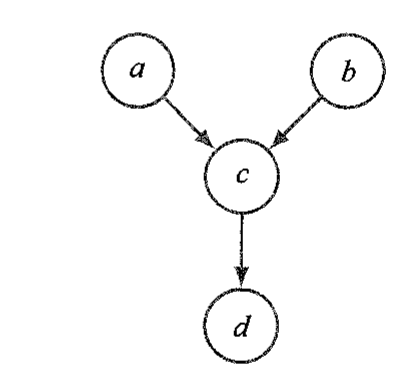
\includegraphics[width=0.34\textwidth]{ch11-fig11-32-descendant.png}
  \caption{当观测到节点$c$的后代节点（即节点$d$）时，用于研究头头相接路径$a$-$c$-$b$的条件独立性的图模型示例}
  \label{figure:ch11-后代节点示例}
\end{figure}

\begin{exercise}\label{exercise:ch11-14}
（$\star$）以\cref{figure:ch11-汽车燃油系统}所示的汽车燃油系统为例，假设驾驶员$D$未直接观测到燃油表$G$的状态，而是看到了燃油表并向我们报告了燃油表读数。该驾驶员报告指出，燃油表要么显示油箱已满（$D=1$），要么显示油箱已空（$D=0$）。该驾驶员有点不可靠，具体由以下概率可以看出：
\begin{align}
  p(D=1\mid G=1) &= 0.9,\\
  p(D=0\mid G=0) &= 0.9.
\end{align}
假设该驾驶员告诉我们燃油表显示油箱已空，换句话说，$D=0$。仅根据这一条件，计算油箱为空的概率。同样，在观测到电池没电的情况下，计算相应的概率，注意第二个概率更低。讨论这一结果，并将该结果与\cref{figure:ch11-后代节点示例}联系起来。
\end{exercise}

\begin{exercise}\label{exercise:ch11-15}
（$\star\star$）用最大似然法训练一个朴素Bayes模型，假设条件为\eqref{align:ch11-朴素Bayes分解}，并假设每个类-条件密度$p(x^{(l)}\mid C_k)$都由它们各自独立的参数$\mathbf{w}^{(l)}$控制。通过最大化与相应类标签数据相关的似然，然后将先验类概率$p(C_k)$设置为每个类中训练数据点的比例，证明最大似然求解涉及使用相应的观测数据向量$\mathbf{x}_1^{(l)},\cdots,\mathbf{x}_N^{(l)}$。
\end{exercise}

\begin{exercise}\label{exercise:ch11-16}
（$\star\star$）考虑与\cref{figure:ch11-一阶Markov链}所示的有向图相对应的联合概率分布[\eqref{align:ch11-一阶Markov}]。利用概率的加和法则与乘积法则，验证在$n=2,\cdots,N$时，该联合概率分布满足条件独立性[\eqref{align:ch11-一阶Markov性质}]。同样，证明形式为\eqref{align:ch11-二阶Markov}的联合分布所描述的二阶Markov模型满足$n=3,\cdots,N$时的条件独立性：
\begin{align}
  p(x_n\mid x_1,\cdots,x_{n-1}) = p(x_n\mid x_{n-1},x_{n-2}).
  \label{align:ch11-二阶Markov性质}
\end{align}
\end{exercise}

\begin{exercise}\label{exercise:ch11-17}
（$\star$）通过使用d分离，验证\cref{figure:ch11-一阶Markov链}所示的一阶Markov模型（其中有$N$个节点）在$n=2,\cdots,N$时满足条件独立性[\eqref{align:ch11-一阶Markov性质}]。同样，证明\cref{figure:ch11-二阶Markov链}所示的二阶Markov模型（其中也有$N$个节点）在$n=3,\cdots,N$时满足条件独立性[\eqref{align:ch11-二阶Markov性质}]。
\end{exercise}

\begin{exercise}\label{exercise:ch11-18}
（$\star$）考虑\cref{figure:ch11-二阶Markov链}所示的二阶Markov过程，通过合并相邻的变量对，证明它可以用新变量的一阶Markov过程来表示。
\end{exercise}

\begin{exercise}\label{exercise:ch11-19}
（$\star$）通过使用d分离，证明\cref{figure:ch11-状态空间模型}中的有向图所代表的状态空间模型的观测数据分布$p(x_1,\cdots,x_N)$不满足任何条件独立性，因此观测变量在任何有限阶都不符合Markov特性。
\end{exercise}

\end{document}
